\documentclass{ansarticle-preprint}
%\usepackage{ucs}
\usepackage[utf8]{inputenc}
\usepackage{amsmath}
%\usepackage{cite}
\usepackage{anslistings}
\usepackage{multicol}
\usepackage{pdfsync}

\usepackage{pgfplots}
\usepackage{pgfplotstable}

\usepackage{fontenc}
\usepackage{graphicx}
\usepackage{xspace}

\usepackage{siunitx}

%\renewcommand{\baselinestretch}{2.0}

\usepackage[normalem]{ulem}

\usepackage{todonotes}

\pgfplotsset{compat=1.9}
\definecolor{gnuplot@lightblue}{RGB}{87,181,232}
\definecolor{gnuplot@green}{RGB}{0,158,115}
\definecolor{gnuplot@purple}{RGB}{148,0,212}

\newcommand{\specialword}[1]{\texttt{#1}}
\newcommand{\dealii}{{\specialword{deal.II}}\xspace}
\newcommand{\pfrst}{{\specialword{p4est}}\xspace}
\newcommand{\trilinos}{{\specialword{Trilinos}}\xspace}
\newcommand{\aspect}{\specialword{Aspect}\xspace}
\newcommand{\petsc}{\specialword{PETSc}\xspace}
\newcommand{\cmake}{{\specialword{CMake}}\xspace}
\newcommand{\autoconf}{{\specialword{autoconf}}\xspace}

%
% Author list -- please add yourself in both places below (in
%                alphabetical order) if you think that your
%                contributions to the last release warrant this
%

\hypersetup{
  pdfauthor={
     Daniel Arndt,
     Wolfgang Bangerth,
     Bruno Blais,
     Thomas C. Clevenger,
%     Denis Davydov,
    Marc Fehling,
%     Daniel Garcia-Sanchez,
    Alexander V. Grayver,
%     Graham Harper,
    Timo Heister,
    Luca Heltai,
    Martin Kronbichler,
    Peter Munch,
%     Ross Maguire Kynch,
    Matthias Maier,
%     Jean-Paul Pelteret,
    Reza Rastak,
    Bruno Turcksin,
    David Wells
    Zhuoran Wang,
  },
  pdftitle={The deal.II Library, Version 9.2, 2020},
}

\title{The \dealii Library, Version 9.2}

 \author[*1]{Daniel Arndt}
 \affil[1]{Computational Engineering and Energy Sciences Group,
   Computional Sciences and Engineering Division,
   Oak Ridge National Laboratory, 1 Bethel Valley Rd.,
   TN 37831, USA.
   \texttt{arndtd@ornl.gov}}

 \author[2]{Wolfgang~Bangerth}
 \affil[2]{Department of Mathematics and Department of Geosciences, Colorado State University, Fort
   Collins, CO 80523-1874, USA.
   \texttt{bangerth@colostate.edu}}


\author[3]{Bruno Blais}
\affil[3]{Research Unit for Industrial Flows Processes (URPEI),
          Polytechnique Montréal,
          PO Box 6079, Stn Centre-Ville, Montréal, Québec, Canada, H3C 3A7.
          {\texttt{bruno.blais@polymtl.ca}}}

 \author[4]{Thomas~C.~Clevenger}
 \affil[4]{School of Mathematical and Statistical Sciences,
   Clemson University,
   Clemson, SC, 29634, USA
   {\texttt{tcleven/heister@clemson.edu}}}
%
% \author[4]{Denis~Davydov}
% \affil[4]{Chair of Applied Mechanics,
%   Friedrich-Alexander-Universit\"{a}t Erlangen-N\"{u}rnberg,
%   Egerlandstr.\ 5,
%   91058 Erlangen, Germany.
%   {\texttt{\{denis.davydov,jean-paul.pelteret\}@fau.de}}}
%
\author[5]{Marc~Fehling}
\affil[5]{Institute for Advanced Simulation,
  Forschungszentrum J\"{u}lich GmbH,
  52425 J\"{u}lich, Germany.
  {\texttt{m.fehling@fz-juelich.de}}}
%
% \author[6]{Daniel Garcia-Sanchez}
% \affil[6]{Sorbonne Universit\'es, UPMC Univ.\ Paris 06, CNRS-UMR 7588,
%   Institut des NanoSciences de Paris, F-75005, Paris, France
%   {\texttt{daniel.garcia-sanchez@insp.upmc.fr}}}
%
% \author[2]{Graham Harper}
%

\author[6]{Alexander~V.~Grayver}
\affil[6]{Institute of Geophysics,
  ETH Zurich,
  Sonneggstrasse 5, 8092 Z\"{u}rich, Switzerland.
  {\texttt{agrayver@ethz.ch}}}

\author[3]{Timo~Heister}

\author[8]{Luca~Heltai}
\affil[8]{SISSA,
   International School for Advanced Studies,
   Via Bonomea 265,
   34136, Trieste, Italy.
   {\texttt{luca.heltai@sissa.it}}}

 \author[9]{Martin~Kronbichler}
 \affil[9]{Institute for Computational Mechanics,
   Technical University of Munich,
   Boltzmannstr.~15, 85748 Garching, Germany.
   {\texttt{kronbichler/munch@lnm.mw.tum.de}}}
%
% \author[10]{Ross~Maguire~Kynch}
% \affil[10]{Zienkiewicz Centre for Computational Engineering,
%   College of Engineering, Swansea University,
%   Bay Campus, Fabian Way, Swansea SA1 8EN, Wales, UK.
%   {\texttt{rkynch@gmail.com}}}
%
\author[11]{Matthias~Maier}
\affil[11]{Department of Mathematics,
  Texas A\&M University,
  3368 TAMU,
  College Station, TX 77845, USA.
  {\texttt{maier@math.tamu.edu}}}

  \author[9,13]{Peter Munch}


 \affil[13]{Institute of Materials Research, Materials Mechanics,
 Helmholtz-Zentrum Geesthacht,
 Max-Planck-Str. 1, 21502 Geesthacht, Germany.
   {\texttt{peter.muench@hzg.de}}}

%
% \author[4]{Jean-Paul~Pelteret}
%
 \author[14]{Reza Rastak}
 \affil[14]{Department of Civil and Environmental Engineering,
   Stanford University,
   Stanford, CA 94305, USA.
   {\texttt{rastak@stanford.edu}}}

\author[*1]{Bruno~Turcksin}
%
\author[12]{David Wells}
\affil[12]{Department of Mathematics, University of North Carolina,
  Chapel Hill, NC 27516, USA.
  {\texttt{drwells@email.unc.edu}}}


\author[14]{Zhuoran Wang}
\affil[14]{Department of Mathematics, Colorado State University, Fort Collins,
          CO 80523-1874, USA.
{\texttt{zhrwang@colostate.edu}}}         
\renewcommand{\labelitemi}{--}


\begin{document}
\maketitle

\footnotetext{%
  $^\ast$ This manuscript has been authored by UT-Battelle, LLC under Contract No.
  DE-AC05-00OR22725 with the U.S. Department of Energy. The United States
  Government retains and the publisher, by accepting the article for
  publication, acknowledges that the United States Government retains a
  non-exclusive, paid-up, irrevocable, worldwide license to publish or reproduce
  the published form of this manuscript, or allow others to do so, for United
  States Government purposes. The Department of Energy will provide public
  access to these results of federally sponsored research in accordance with the
  DOE Public Access Plan (http://energy.gov/downloads/doe-public-access-plan).}

\begin{abstract}
  This paper provides an overview of the new features of the finite element
  library \dealii, version 9.2.
\end{abstract}



%%%%%%%%%%%%%%%%%%%%%%%%%%%%%%%%%%%%%%%%%%%%%%%%%%%%%%%%%%%%%%%%%%%%%%%%%%%%%%%%
%%%%%%%%%%%%%%%%%%%%%%%%%%%%%%%%%%%%%%%%%%%%%%%%%%%%%%%%%%%%%%%%%%%%%%%%%%%%%%%%
%%%%%%%%%%%%%%%%%%%%%%%%%%%%%%%%%%%%%%%%%%%%%%%%%%%%%%%%%%%%%%%%%%%%%%%%%%%%%%%%
\section{Overview}

\dealii version 9.2.0 was released May XYZ, 2020.
This paper provides an
overview of the new features of this release and serves as a citable
reference for the \dealii software library version 9.2. \dealii is an
object-oriented finite element library used around the world in the
development of finite element solvers. It is available for free under the
GNU Lesser General Public License (LGPL). Downloads are available at
\url{https://www.dealii.org/} and \url{https://github.com/dealii/dealii}.

The major changes of this release are:
%
\begin{itemize}
\item xy \todo[inline]{Update once we have the subsections in Section 2;
  provide cross-references to each of these subsections}
%   \item Improved support for automatic differentiation (see
%     Section~\ref{subsec:ad}),
\end{itemize}
%
These major changes are discussed in detail in Section~\ref{sec:major}. There
are a number of other noteworthy changes in the current \dealii{} release
that we briefly outline in the remainder of this section:
%
\begin{itemize}
\item \dealii{} had decent support for solving complex-valued problems
  (e.g., ones in quantum mechanics -- like the example covered by the
  \texttt{step-58} tutorial program covered below -- or for
  time-harmonic problems) for a while already. However, there were two
  areas in which support was missing. First, the UMFPACK direct solver
  packaged with \dealii{} did not support solving complex-valued
  linear problems. This has now been addressed: UMFPACK actually can
  solve such systems, we just needed to write the appropriate
  interfaces. Second, the \texttt{DataOut} class that is responsible
  for converting nodal data into information that can then be written
  into files for visualization did not know how to deal with vector-
  and tensor-valued fields whose components are complex numbers. An
  example for this is to solve the time-harmonic version of the
  Maxwell equations that has the electric and magnetic fields as
  solution. This, too, has been addressed in this release.
\item The class \texttt{DiscreteTime} is introduced to provide a more
  consistent, more readable, and less error-prone approach to control
  time-stepping algorithms within time-dependent simulations.
  The mutating interface of this class is designed to be minimal
  to enforce a number of important programming invariants, reducing
  the possibility of mistakes in the user code.
  When time-incrementation is requested within the user code, the class makes
  sure that time increases by a non-zero step size and the current step
  number is incremented accordingly.
  Furthermore, \texttt{DiscreteTime} ensures that the final time step ends
  precisely on a predefined end time. Therefore, the final step size is
  automatically lengthened or shortened to accommodate this feature.
  In addition, the class provides useful access methods which return the step
  number $n$, the values of the simulation time corresponding to $t_{n-1}$,
  $t_n$, and $t_{n+1}$, and the step-size values $t_n - t_{n-1}$ and
  $t_{n+1} - t_n$.
\item z \todo[inline]{What else? Maybe mention the updated step-12?}
\end{itemize}
%
In addition to these changes, the changelog lists more than 200 other
features and bugfixes.




%%%%%%%%%%%%%%%%%%%%%%%%%%%%%%%%%%%%%%%%%%%%%%%%%%%%%%%%%%%%%%%%%%%%%%%%%%%%%%%%
%%%%%%%%%%%%%%%%%%%%%%%%%%%%%%%%%%%%%%%%%%%%%%%%%%%%%%%%%%%%%%%%%%%%%%%%%%%%%%%%
%%%%%%%%%%%%%%%%%%%%%%%%%%%%%%%%%%%%%%%%%%%%%%%%%%%%%%%%%%%%%%%%%%%%%%%%%%%%%%%%
\section{Major changes to the library}
\label{sec:major}

This release of \dealii contains a number of large and significant changes
that will be discussed in this section.

It of course also contains a
vast number of smaller changes and added functionality; the details of these
can be found
\href{https://dealii.org/developer/doxygen/deal.II/changes_between_9_0_1_and_9_1_0.html}{
in the file that lists all changes for this release}, see \cite{changes91}.


%%%%%%%%%%%%%%%%%%%%%%%%%%%%%%%%%%%%%%%%%%%%%%%%%%%%%%%%%%%%%%%%%%%%%%%%%%%%%%%%
\subsection{A new fully distributed triangulation class}
\label{subsec:pft}

By release 9.1, all triangulation classes of \texttt{deal.II} have in common that the coarse grid is shared by
all processes and the actual mesh used for computations is constructed by repeated
refinement. However, this has its limitations in industrial applications where, often, the mesh comes
from an external mesh generator in the form of a file that already contains millions
or tens of millions of cells. For such configurations, applications might exhaust
available memory already while reading the mesh on each MPI process.

The new class \texttt{parallel::fullydistributed::Triangulation} targets this issue
by distributing also the coarse grid. Such
a triangulation can be created by providing to each process a \texttt{Triangulation\-De\-scrip\-tion::Description} struct, containing
1) the relevant data to construct the local part of the coarse grid, 2) the
translation of the local coarse-cell IDs to globally unique IDs, 3) the hierarchy
of mesh refinements, and 4) the owner of the cells on the active mesh level as well
as on the multigrid levels. For the current release, triangulations is set up
this way cannot be adaptively refined after construction, which is planned to be
improved for the next release.

%The \texttt{TriangulationDescription::Description} struct can be filled manually or
%by the utility functions from the \texttt{TriangulationDescription::Utilities}
%namespace. The function \texttt{create\_\allowbreak description\_\allowbreak
%from\_ \allowbreak triangulation()} can convert a base triangulation (partitioned
%serial \texttt{Tri\-angulation} and \texttt{parallel::distributed::Triangulation})
%to such a struct. The advantage of this approach is that all known utility
%functions from the namespaces \texttt{GridIn} and \texttt{GridTools} can be used
%on the base triangulations before converting them to the structs. Since this
%function suffers from the same main memory problems as described above, we also
%provide the function \texttt{create\_description\_from\_triangulation\_in\_groups()},
%which creates the structs only on the master process in a process group. These
%structs are filled one by one and are sent to the relevant processes once they are
%ready. A sensible process group size might contain all processes of one compute node.


The new fully distributed triangulation class supports 1D, 2D, and 3D meshes
including geometric multigrid hierarchies, periodic boundary conditions, and
hanging nodes.

%We intend to extend the usability of the new triangulation class in regard of
%different aspects, e.g., I/O. In addition, we would like to enable adaptive mesh
%refinement, a feature of the other triangulation classes, which is very much
%appreciated by many users. For repartitioning, we plan to use an oracle approach
%known from \texttt{parallel::distributed::Triangulation}. Here, we would like to
%rely on a user-provided partitioner, which might also be a graph partitioner.



%%%%%%%%%%%%%%%%%%%%%%%%%%%%%%%%%%%%%%%%%%%%%%%%%%%%%%%%%%%%%%%%%%%%%%%%%%%%%%%%
\subsection{Improved large-scale performance}
\label{subsec:performance}

Large-scale simulations with 304,128 cores have revealed bottlenecks in release
9.1 during initialization of a number of distributed data structures due to the usage of expensive collective operations
like \texttt{MPI\_Allgather()} and \texttt{MPI\_\allowbreak
  Alltoall()}. Typical examples are the
pre-computation of those indices of the vector entries (or
other linear index ranges) owned by
each process, which were previously stored in  an array on every process.
This information is needed to set up
the  \texttt{Utilities::MPI::Par\-ti\-ti\-oner} class.
In release 9.2, we have replaced these functions in favor of
consensus algorithms~\cite{hoefler2010scalable}, which can be
found in the namespace \texttt{Utilities::\allowbreak MPI::\allowbreak ConsensusAlgorithms} (short: \texttt{CA}).
Now, only the locally relevant information about the index ranges is
(re)computed when needed, which, for more than 100 MPI processes, uses
point-to-point communications and a single \texttt{MPI\_IBarrier()}.

%Consensus algorithms are algorithms dedicated to efficient dynamic-sparse
%communication patterns. In this context, the term ``dynamic-sparse'' means
%that by the time this function is called, the other processes do not know
%yet that they have to answer requests and
%each process only has to communicate with a small subset of processes of the
%MPI communicator. We provide two flavors of the consensus algorithm: the two-step
%approach \texttt{ConsensusAlgorithms::PEX} and the \texttt{ConsensusAlgorithms::NBX},
%which uses only point-to-point communications and a single \texttt{MPI\_IBarrier()}.
%The class \texttt{ConsensusAlgorithms::Selector} selects one of the two previous
%algorithms, depending on the number of processes.

Users can apply the new algorithms for their own dynamic-sparse problems by
providing a list of target
processes and pack/unpack routines either by implementing the interface
\texttt{CA::\allowbreak Process} or by providing \texttt{std::function}
objects to \texttt{CA::AnonymousProcess}.

\todo[inline]{Aren't the target processes the result of the operation, and the
  input global numbers of indices that we request?}

By replacing the collective communications during set up and removing the arrays
that contain information for each process (enabled by the application of consensus
algorithms and other modifications---a full list of modifications leading to this
improvement can be found online), we were able to significantly
improve the set up
time for large-scale simulations and to solve a Poisson problem with multigrid
with \num{2.1e12} unknowns.
Figure~\ref{fig:init_costs} compares the timings of simulations of various problem
sizes (including set up) on 49,152 MPI ranks using a matrix-free solver according
to~\cite{KronbichlerKormann2019,KronbichlerWall2018} discontinuous elements of
degree $5$ in a geometric multigrid (GMG) scheme with the previous release 9.1
and with the current release 9.2. While the scaling for the V-cycle had been
very good before, many initialization routines have been considerably
improved, especially the enumeration of unknowns on the multigrid levels and
the setup of the multigrid transfer.

\pgfplotstableread{
dofs  grid  distdofs  mfsetup  mgtransfer  smoother  vcycle
14155776  0.347457  0.02424084  0.03346427  0.0105426  0.0108817  0.0035033
28311552  0.35134  0.0215024  0.0340963  0.0095201  0.010616  0.0035887
56623104  0.41577  0.0243593  0.0432297  0.011557  0.011667  0.0041244
113246208  0.42172  0.0323919  0.0427806  0.012983  0.011834  0.0043853
226492416  0.43565  0.0404079  0.0421606  0.012867  0.017305  0.0056340
452984832  0.5055  0.0500101  0.0562977  0.017739  0.022763  0.0061992
905969664  0.54552  0.065865  0.0641994  0.019445  0.037431  0.0087932
1811939328  0.5672  0.104909  0.080807  0.025395  0.063548  0.0133252
3623878656  0.65541  0.165071  0.129717  0.042294  0.12644  0.0218619
7247757312  0.74521  0.251417  0.221072  0.073314  0.21807  0.0339264
14495514624  0.84789  0.403463  0.36894  0.11425  0.4091  0.0669798
28991029248  0.91983  0.52435  0.5363  0.14189  0.79178  0.1322448
57982058496  1.0339  0.87448  0.93134  0.23863  1.5896  0.2539445
115964116992  1.2667  1.46016  1.70806  0.44101  3.1409  0.4956625
231928233984  1.7597  2.58121  3.3741  0.77624  6.2628  0.9857200
}\tableinit

\pgfplotstableread{
dofs  grid  distdofs  mfsetup  mgtransfer  smoother  vcycle
14155776  2.0148  0.9086  0.433886  1.3099  0.010685  0.0035033
28311552  1.8746  0.91078  0.576777  1.3093  0.010752  0.0035887
56623104  2.0924  0.98058  0.574183  1.4459  0.011831  0.0041244
113246208  2.3788  1.22025  0.547492  1.7919  0.011979  0.0043853
226492416  2.1254  1.50329  0.839219  1.7832  0.017819  0.0056340
452984832  2.4325  2.10171  0.711708  2.0263  0.023393  0.0061992
905969664  3.8911  3.58355  1.08478  2.5844  0.045697  0.0087932
1811939328  4.1803  4.379  0.784804  1.8947  0.061552  0.0133252
3623878656  2.6654  5.6073  0.833896  1.8912  0.1188  0.0218619
7247757312  2.7422  7.8463  0.741733  1.8477  0.21291  0.0339264
14495514624  2.765  9.9848  0.99218  1.8248  0.40665  0.0669798
28991029248  3.2901  15.0526  1.5124  2.6723  0.81013  0.1322448
57982058496  3.1927  21.0562  1.72831  2.1998  1.5905  0.2539445
115964116992  4.1485  31.0087  2.67998  2.9091  3.2009  0.4956625
231928233984  4.1787  47.195  4.2821  3.9558  6.3362  0.9857200
}\tableinitold

\begin{figure}
  \begin{tikzpicture}
    \begin{loglogaxis}[
      width=0.51\textwidth,
      height=0.38\textwidth,
          xlabel={\# DoFs},
          ylabel={time [s]},
          title={9.1 release},
          xtick={1.4e7,5.7e7,2.3e8,9.1e8,3.6e9,1.4e10,5.8e10,2.3e11},
          xticklabels={1.4$\times 10^7$,5.7$\times 10^7$,2.3$\times 10^8$,9.1$\times 10^8$,3.6$\times 10^9$,1.4$\times 10^{10}$,5.8$\times 10^{10}$,2.3$\times 10^{11}$},
          tick label style={font=\scriptsize},
          xticklabel style={rotate=25,anchor=north east},
          label style={font=\scriptsize},
          legend style={font=\scriptsize},
          %legend to name=legend:scalingMG,
          %legend cell align=left,
          %legend columns = 3,
          ymin=2e-3,ymax=8e1,
          grid, thick]
          \addplot table[x index = 0, y index={1}] {\tableinitold};
          \addplot[red,mark=square*] table[x index = 0, y index={2}] {\tableinitold};
          \addplot[gnuplot@green,mark=otimes] table[x index = 0, y index={3}] {\tableinitold};
          \addplot[gnuplot@lightblue,mark=triangle] table[x index = 0, y index={4}] {\tableinitold};
          \addplot[gnuplot@purple,mark=diamond] table[x index = 0, y index={5}] {\tableinitold};
          \addplot[black,mark=x] table[x index = 0, y index={6}] {\tableinitold};
    \end{loglogaxis}
  \end{tikzpicture}
  \hfill
  \begin{tikzpicture}
    \begin{loglogaxis}[
      width=0.51\textwidth,
      height=0.38\textwidth,
          xlabel={\# DoFs},
          ylabel={time [s]},
          title={9.2 release},
          xtick={1.4e7,5.7e7,2.3e8,9.1e8,3.6e9,1.4e10,5.8e10,2.3e11},
          xticklabels={1.4$\times 10^7$,5.7$\times 10^7$,2.3$\times 10^8$,9.1$\times 10^8$,3.6$\times 10^9$,1.4$\times 10^{10}$,5.8$\times 10^{10}$,2.3$\times 10^{11}$},
          tick label style={font=\scriptsize},
          xticklabel style={rotate=25,anchor=north east}, thick,
          label style={font=\scriptsize},
          legend style={font=\scriptsize},
          legend to name=legend:init,
          legend cell align=left,
          legend columns = 6,
          ymin=2e-3,ymax=8e1,
          grid]
          \addplot table[x index = 0, y index={1}] {\tableinit};
          \addlegendentry{create mesh};
          \addplot[red,mark=square*] table[x index = 0, y index={2}] {\tableinit};
          \addlegendentry{enumerate (mg) dofs};
          \addplot[gnuplot@green,mark=otimes] table[x index = 0, y index={3}] {\tableinit};
          \addlegendentry{init matrix-free};
          \addplot[gnuplot@lightblue,mark=triangle] table[x index = 0, y index={4}] {\tableinit};
          \addlegendentry{init GMG transfer};
          \addplot[gnuplot@purple,mark=diamond] table[x index = 0, y index={5}] {\tableinit};
          \addlegendentry{init smoother};
          \addplot[black,mark=x] table[x index = 0, y index={6}] {\tableinit};
          \addlegendentry{GMG V-cycle};
    \end{loglogaxis}
  \end{tikzpicture}
  \\
  \strut\hfill\pgfplotslegendfromname{legend:init}\hfill\strut
  \caption{Comparison of initialization costs of various data structures in the 9.1 release (left) and the new 9.2 release (right) when run on 49,152 MPI ranks.}
  \label{fig:init_costs}
\end{figure}


The new code has been also applied to solve problems with adaptively refined
meshes with more than \num{4e9} unknowns. {\color{red}TODO[Timo]}

\todo[inline]{We did solve adaptive problems with more than 4B unknowns before, but some were broken for a while during this release stage due to the consensus algorithms. But we did not test systems or block vectors before. But we should not make it sound too negative.}


%%%%%%%%%%%%%%%%%%%%%%%%%%%%%%%%%%%%%%%%%%%%%%%%%%%%%%%%%%%%%%%%%%%%%%%%%%%%%%%%
\subsection{Better support for parallel $hp$-adaptive algorithms}
\label{subsec:hp}

With the previous release, \dealii supports $hp$-adaptive finite element methods
on distributed memory systems \cite{dealII91}. We implemented the bare functionality
for $hp$-adaptive methods with the objective to offer the greatest flexibility in
their application. Here, reference finite elements still had to be assigned manually
to each cell, which may not lead to an optimal mesh and is tedious.

With the current release, $hp$-adaptive finite element methods have been further
expanded: New features like decision strategies have been added and the user interface
has been overhauled, effectively making $hp$-methods more attractive to use. We introduced
many new functions that automatize the general workflow for applying $hp$-decision
strategies, which run on top of the previous low-level implementation for both serial
and parallel applications.

The interface is now as simple to use as the one for pure adaptive mesh refinement.
Consider the following (incomplete) listing as an example: We estimate both error and
smoothness of the finite element approximation. Further, we flag certain fractions of
cells with the highest and lowest errors for refinement and coarsening, respectively
(here: 30\% / 3\%). From those cells listed for adaptation, we specify a subset of them
for $h$- and $p$-adaptation (here: 10\% / 90\%).
\begin{c++}
Vector<float> estimated_error_per_cell (n_active_cells);
KellyErrorEstimator::estimate(
  dof_handler, ..., solution, estimated_error_per_cell, ...);
GridRefinement::refine_and_coarsen_fixed_number(
  triangulation, estimated_error_per_cell, 0.3, 0.03);

Vector<float> estimated_smoothness_per_cell (n_active_cells);
SmoothnessEstimator::Legendre::coefficient_decay(
  ..., dof_handler, solution, estimated_smoothness_per_cell);
hp::Refinement::p_adaptivity_fixed_number(
  dof_handler, estimated_smoothness_per_cell, 0.9, 0.9);
hp::Refinement::choose_p_over_h (dof_handler);

triangulation.execute_coarsening_and_refinement();
\end{c++}

In particular, we implemented decision strategies based on refinement history and
smoothness estimation, and made sure that they work for refinement as well as
coarsening in terms of $h$- and $p$-adaptation in serial and parallel applications.

The former relies on knowing an estimate for the upper error bound \cite[Thm.~3.4]{BabuskaSuri1990}.
For successive refinements, we can predict how the error will change on basis of
current error estimates and adaptation flags. In the next refinement cycle, these
predicted error estimates allow us to decide whether the choice of adaptation in
the previous cycle was justified, and provide the foundation for it in the next
one \cite{MelenkWohlmuth2001}.

In general, $p$-refinement is favorable over $h$-refinement in smooth regions of
the finite element approximation \cite[Thm.~3.4]{BabuskaSuri1990}. Thus, estimating
its smoothness provides a suitable decision indicator for $hp$-adaptation. For this
purpose, we express the finite element approximation in an orthogonal
basis of increasing frequency, and consider the decay of their expansion
coefficients as the estimation of smoothness. This has been implemented for both
Fourier coefficients \cite{BangerthKayserHerold2007} and Legendre coefficients
\cite{Mavriplis1994,HoustonSeniorSueli2003,HoustonSueli2005,EibnerMelenk2007}.


%%%%%%%%%%%%%%%%%%%%%%%%%%%%%%%%%%%%%%%%%%%%%%%%%%%%%%%%%%%%%%%%%%%%%%%%%%%%%%%%
\subsection{Support for particle-based methods}
\label{subsec:particles}

\todo[inline]{Luca: Your section}


%%%%%%%%%%%%%%%%%%%%%%%%%%%%%%%%%%%%%%%%%%%%%%%%%%%%%%%%%%%%%%%%%%%%%%%%%%%%%%%%
\subsection{Improved performance of the symbolic differentiation framework}
\label{subsec:symbdiff}

\todo[inline]{J-P's section}

BatchOptimizer for symbolic expressions
\begin{itemize}
\item CSE for dictionary-based expressions
\item ``lambdify'' (via SymEngine)
\item Offloading to LLVM JIT compiler (via SymEngine)
\item Serialization, so complex expressions can be compiled offline
\end{itemize}


%%%%%%%%%%%%%%%%%%%%%%%%%%%%%%%%%%%%%%%%%%%%%%%%%%%%%%%%%%%%%%%%%%%%%%%%%%%%%%%%
\subsection{Advances of the SIMD capabilities and the matrix-free infrastructure}
\label{subsec:mf}

%\begin{itemize}
%\item ECL
%\item VectorizedArrayType
%\end{itemize}

The class \texttt{VectorizedArray<Number>} is a key ingredient for the high
node-level performance of the matrix-free algorithms in deal.II~\cite{KronbichlerKormann2012, KronbichlerKormann2019}. It is a wrapper
class around a short vector of $n$ entries of type \texttt{Number} and maps
arithmetic operations to appropriate single-instruction/multiple-data (SIMD)
concepts by intrinsic functions.
The class \texttt{VectorizedArray} has been made more user-friendly in this release by making
it compatible with the STL algorithms found in the header \texttt{<algorithm>}.
The length of the  vector can now be queried by  \texttt{VectorizedArray::size()} and its underlying number type by \texttt{VectorizedArray::value\_type}.
Furthermore, the \texttt{VectorizedArray} class now supports range-based iterations over its entries.

Up to release 9.1, the
vector length $n$ has been set at compile time of the library to the highest
possible value supported by the given processor architecture.
Now, a second optional template argument
\texttt{VectorizedArray<Number, size>} can be given with \texttt{size} explicitly controlling
the vector length within the capabilities of a particular instruction set.
A full list of supported
vector lengths is presented in Table~\ref{tab:vectorizedarray}.

To account for the variable-size \texttt{VectorizedArray} class, all matrix-free related classes (like \texttt{MatrixFree} and \texttt{FEEvaluation})
have been extended with a new optional template argument specifying the
\texttt{VectorizedArrayType}. This allows users to select the vector length/ISA and,
as a consequence, the number of cells to be processed at once directly in their applications:
The deal.II-based
library \texttt{hyper.deal}~\cite{munch2020hyperdeal}, which solves the 6D Vlasov--Poisson equation with high-order
discontinuous Galerkin methods (with more than a thousand degrees of freedom per cell), constructs a tensor product of two \texttt{MatrixFree} objects of different SIMD-vector
length in the same application and benefits---in terms of performance---by the possibility of decreasing the number of cells processed by a single SIMD instruction.


\begin{table}
\caption{Supported vector lengths of the class \texttt{VectorizedArray} and
the corresponding instruction-set-architecture extensions. }\label{tab:vectorizedarray}
\centering
\begin{tabular}{ccc}
\toprule
\textbf{double} & \textbf{float} & \textbf{ISA}\\
\midrule
VectorizedArray<double, 1> & VectorizedArray<float, 1> & (auto-vectorization) \\
VectorizedArray<double, 2> & VectorizedArray<float, 4> & SSE2/AltiVec \\
VectorizedArray<double, 4> & VectorizedArray<float, 8> & AVX/AVX2 \\
VectorizedArray<double, 8> & VectorizedArray<float, 16> & AVX-512 \\
\bottomrule
\end{tabular}

\caption{Comparison of relevant SIMD-related classes in deal.II and \texttt{C++23}.}\label{tab:simd}
\centering
\begin{tabular}{cc}
\toprule
\textbf{VectorizedArray (deal.II)} & \textbf{std::simd (\texttt{C++23})} \\
\midrule
VectorizedArray<Number> & std::experimental::native\_simd<Number> \\
VectorizedArray<Number, size> & std::experimental::fixed\_size\_simd<Number, size> \\ \bottomrule
\end{tabular}
\end{table}

Furthermore, the new interfaces enable using any data structure
\texttt{VectorizedArrayType} as long as it supports required
functionalities like \texttt{size()} or \texttt{value\_type}. This prepares
for the \texttt{C++23} feature \texttt{std::simd} that will be enabled in the future.
Table~\ref{tab:simd} gives a comparison of the deal.II-specific SIMD classes and
the equivalent \texttt{C++23} classes. Finally, this change also prepares for specialized
code paths exploiting
vectorization within an element~\cite{KronbichlerKormann2019} in the future.

%We welcome the standardization of the SIMD
%parallelization paradigm in C++ and intend to replace step by step our own
%wrapper class, which has been continuously developed over the last decade. We
%would like to emphasize that the work invested in this class was not in vain,
%since many performance-relevant utility functions implemented with \texttt{VectorizedArray} in mind (e.g., \texttt{vectorized\_load\_and\_transpose}
%and \texttt{vectorized\_transpose\_and\_store}) will be still used, since they
%have not become part of the standard.

%Further additions to the \texttt{MatrixFree} infrastructure consist of:
%\begin{itemize}
%\item a new variant of \texttt{MatrixFree::cell\_loop()}: It takes two
%\texttt{std::function} objects with ranges on the locally owned degrees of freedom, one
%with work to be scheduled before the cell operation first touches some
%unknowns and another with work to be executed after the cell operation last
%touches them. The goal of
%these functions is to bring vector operations close to the time when the
%vector entries are accessed by the cell operation, which increases the cache
%hit rate of modern processors by improved temporal locality.
%\item a new form of loop \texttt{MatrixFree::loop\_cell\_centric()}: This
%kind of loop can be used in the context of discontinuous Galerkin methods,
%where both cell and face integrals have to be evaluated. While in the case of
%the traditional \texttt{loop}, cell and face integrals have been performed
%independently, the new loop performs all cell and face integrals of a cell in
%one go. This includes that each face integral has to be evaluated twice, but
%entries have to be written into the solution vector only once with improved
%data locality. Previous publications based on \texttt{deal.II} have shown the
%relevance of the latter aspect for reaching higher performance.
%\end{itemize}


%%%%%%%%%%%%%%%%%%%%%%%%%%%%%%%%%%%%%%%%%%%%%%%%%%%%%%%%%%%%%%%%%%%%%%%%%%%%%%%%
\subsection{Advances in GPU support}
\label{subsec:gpu}

\begin{itemize}
\item overlapping of computation and communication in the case of CUDA-aware MPI
\end{itemize}


%%%%%%%%%%%%%%%%%%%%%%%%%%%%%%%%%%%%%%%%%%%%%%%%%%%%%%%%%%%%%%%%%%%%%%%%%%%%%%%%
\subsection{Expanded use of C++11 facilities}
\label{subsec:cxx}

Certain types of quantities in a simulation are constants fully known
at compile time. They can be pre-calculated and fully stored inside the
compiled program binary in order to avoid unnecessary initialization during
runtime. This optimization is now enabled for the class templates
\texttt{Tensor} and \texttt{SymmetricTensor} by qualifying their constructor,
member functions, and overloaded operators as \texttt{constexpr}.
For instance, the linear mechanical constitutive model for elastic solids
uses a constant fourth-order elasticity tensor
$\mathbb{C} = \lambda \boldsymbol{I} \otimes \boldsymbol{I} + 2 \mu \mathbb{I}$
which does not depend on the current state of strain.
This tensor can be statically initialized by defining it as
\texttt{constexpr SymmetricTensor<4, dim>}.
As another example, the lattice vectors in a crystal plasticity model are generally
constant and known during compilation time, enabling their efficient definition as
\texttt{constexpr Tensor<1, dim>}.
The capability of defining \texttt{constexpr} variables, functions, and methods
was introduced by the C++11 standard and was later expanded by the C++14 standard.
Therefore, the extent of \texttt{constexpr} support in \dealii{} depends on the C++
standard which is used to compile the library. The next release of \dealii{}
will fully adopt the features of the C++14 standard.


%%%%%%%%%%%%%%%%%%%%%%%%%%%%%%%%%%%%%%%%%%%%%%%%%%%%%%%%%%%%%%%%%%%%%%%%%%%%%%%%
\subsection{New and improved tutorial and code gallery programs}
\label{subsec:steps}

Many of the \dealii{} tutorial programs were revised in a variety of
ways as part of this release. A particular example is that we have
converted a number of programs to use range-based for loops (a C++11
feature) for loops over a range of integer indices such as loops over
all quadrature points or all indices of degrees of freedom during
assembly. This makes sense given that the
range-based way of writing loops seems to be the idiomatic approach
these days, and that we had previously already converted loops over
all cells in this way.

In addition, there are a number of new tutorial programs:
\begin{itemize}
\item \texttt{step-47}
\todo[inline]{Zhuoran to write}
\item \texttt{step-50}
  \todo[inline]{Timo/Conrad/... to write}

\item \texttt{step-58} is a program that solves the nonlinear
  Schr{\"o}dinger equation, which in non-dimensional form reads
  \begin{align*}
  - i \frac{\partial \psi}{\partial t}
  - \frac 12 \Delta \psi
  + V \psi
  + \kappa |\psi|^2 \psi
  &= 0,
  \end{align*}
  augmented by appropriate initial and boundary conditions and using
  an appropriate form for the potential $V=V(\mathbf x)$. The
  tutorial program focused on two specific aspects for which this
  equation serves as an excellent test case: (i) Solving
  complex-valued problems without splitting the equation into its
  real and imaginary parts (as \texttt{step-29} does, for
  example). (ii) Using operator splitting techniques. The equation is
  a particularly good test case for this technique because the only
  nonlinear term, $\kappa |\psi|^2 \psi$, does not contain any
  derivatives and consequently forms an ODE to be solved at each time
  step in an operator splitting scheme (for which, furthermore, there
  exists an analytic solution), whereas the remainder of the
  equation is linear and easily solved using standard finite element
  techniques.

\item \texttt{step-65} presents \texttt{TransfiniteInterpolationManifold}, a
manifold class that can propagate curved boundary information into the
interior of a computational domain by transfinite interpolation \cite{Gordon82}.
This manifold is a prototype for many other manifolds in that it is relatively
expensive to compute the new points, especially for higher order mappings. Since
typical programs query higher-order geometries in a large variety of contexts,
the contribution of the mapping to the run time can be significant. As a
solution, the tutorial also presents the class \texttt{MappingQCache}, which
samples the information of expensive manifolds in the points of a
\texttt{MappingQ} and caches it. The tutorial shows that this makes all queries
to the geometry very cheap.

\item \texttt{step-67} is an explicit time integrator for the
compressible Euler equations discretized with a high-order discontinuous
Galerkin scheme using the matrix-free infrastructure. Besides the use of
matrix-free evaluators for systems of equations and over-integration, it also
presents \texttt{MatrixFreeOperators::CellwiseInverseMassMatrix}, a fast implementation
of the action of the inverse mass matrix in the DG setting using tensor
products. Furthermore, this tutorial demonstrates the usage of new
pre and post operations, which can be passed to
\texttt{MatrixFree::cell\_loop()}, to schedule operations on sections of vectors close
to the matrix-vector product to increase data locality.

\item \texttt{step-69}
  \todo[inline]{Matthias/Ignacio to write}

\item \texttt{step-70}
  \todo[inline]{Luca, please write.}
\end{itemize}

\todo[inline]{Do we have new code gallery programs?}

%%%%%%%%%%%%%%%%%%%%%%%%%%%%%%%%%%%%%%%%%%%%%%%%%%%%%%%%%%%%%%%%%%%%%%%%%%%%%%%%
\subsection{Python interfaces}
\label{subsec:python}

\begin{figure}
\renewcommand\figurename{Listing}

\centering

\begin{python}
import PyDealII.Release as dealii

triangulation = dealii.Triangulation('2D')
triangulation.generate_hyper_shell(center = dealii.Point([0, 0]),
                    inner_radius = 0.5, outer_radius = 1.,
                    n_cells = 0, colorize = True)

triangulation.refine_global(2)

for cell in triangulation.active_cells():
    cell.material_id = 1 if cell.center().x > 0 else 2

    for face in cell.faces():
        if face.at_boundary() and\
           face.boundary_id == 1:
            cell.refine_flag ='isotropic'

triangulation.execute_coarsening_and_refinement()
\end{python}

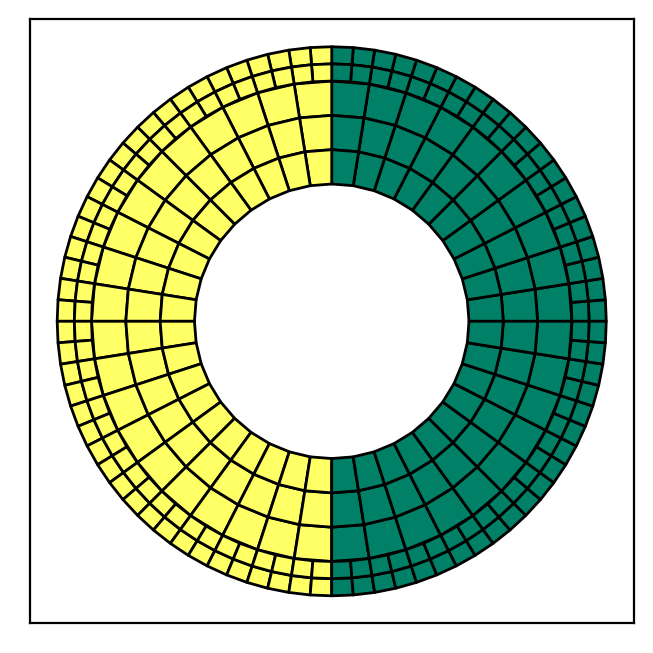
\includegraphics{python_mesh.png}

\caption{Python code that uses \texttt{deal.II}'s Python interface to generate a mesh shown at the bottom (coloured by the cell's material id).}
\label{python_wrapper}
\end{figure}


The initial support for Python has come in \texttt{deal.II 9.0}. The present release significantly extends the Python interface. Specficically, a large number of methods from the C++ classes such as \texttt{Triangulation, CellAccessor, TriaAccessor, Mapping, Manifold, GridTools} can now be invoked from within the Python. The accent was made on methods and functions that are widely used at a mesh preparation stage when a mesh is created and parameters related to the boundary, manifold and material identifiers are assigned.

A triangulation object can be read in or created using a number of simplistic geometries offered by the \texttt{GridGenerator}'s functions. Further information such as boundary, material and manifold identifiers can be assigned to cells and respective faces or edges (see Listing \ref{python_wrapper}). The introspective nature of the Python language makes it easy to infer the list of supported methods from the Python objects, for example by typing \texttt{dir(PyDealII.Release.Triangulation)}.

All triangulations created within the Python are serial. Once the mesh is designed, triangulation can be serialized along with the auxiliary information about possible refinement, boundaries, materials and manifolds. This object can be easily deserialized within a C++ program for subsequent production runs. Although saved triangulations are serial, it is possible to use them for construction of \texttt{parallel::shared, parallel::disrtibuted, and parallel::fullydistributed} (see also Section \ref{subsec:pft}) types of triangulations respecting the refinement and all the auxiliary information.

To facilitate the illustration of the new Python bindings, tutorial programs \href{https://github.com/dealii/dealii/blob/dealii-9.2/examples/step-49/step-49.ipynb}{step-49} and \href{https://github.com/dealii/dealii/blob/dealii-9.2/examples/step-53/step-53.ipynb}{step-53} were replicated in a form of the Jupyter notebooks.

Note that the current Python interface does not yet provide access to the actual \texttt{deal.II}'s finite element machinery, that is classes such as \texttt{DoFHandler, FE\_*, FEValues}, etc. It is envisaged that a progress towards this will be made for the next release.

%%%%%%%%%%%%%%%%%%%%%%%%%%%%%%%%%%%%%%%%%%%%%%%%%%%%%%%%%%%%%%%%%%%%%%%%%%%%%%%%
\subsection{Incompatible changes}

The 9.2 release includes
\href{https://dealii.org/developer/doxygen/deal.II/changes_between_9_1_1_and_9_2_0.html}
     {around 60 incompatible changes}; see \cite{changes92}. The majority of these changes
should not be visible to typical user codes; some remove previously
deprecated classes and functions; and the majority change internal
interfaces that are not usually used in external
applications. However, some are worth mentioning:
\begin{itemize}
\item Two functions that provide information about all processes,
  namely
  \begin{itemize}
 \item \texttt{DoFHandler::locally\_owned\_dofs\_per\_processor()}
 \item \texttt{DoFHandler::locally\_owned\_mg\_dofs\_per\_processor()}
  \end{itemize}
have been deprecated. As discussed in
Subsection~\ref{subsec:performance}, deal.II by default no longer
stores information for all processes on all processes, but only the
local information or the locally-relevant information. On the other
hand, if necessary, global information can still be computed using,
for example, calling \texttt{Utilities::MPI::Allgather(locally\_owned\_info(), comm)}.
\item
  \todo[inline]{What else is worth mentioning? Someone needs to go
    through the list of incompatible changes...}
\end{itemize}



%%%%%%%%%%%%%%%%%%%%%%%%%%%%%%%%%%%%%%%%%%%%%%%%%%%%%%%%%%%%%%%%%%%%%%%%%%%%%%%%
%%%%%%%%%%%%%%%%%%%%%%%%%%%%%%%%%%%%%%%%%%%%%%%%%%%%%%%%%%%%%%%%%%%%%%%%%%%%%%%%
%%%%%%%%%%%%%%%%%%%%%%%%%%%%%%%%%%%%%%%%%%%%%%%%%%%%%%%%%%%%%%%%%%%%%%%%%%%%%%%%
\section{How to cite \dealii}\label{sec:cite}

In order to justify the work the developers of \dealii put into this
software, we ask that papers using the library reference one of the
\dealii papers. This helps us justify the effort we put into it.

There are various ways to reference \dealii. To acknowledge the use of
the current version of the library, \textbf{please reference the present
document}. For up to date information and a bibtex entry for this document
see:
\begin{center}
 \url{https://www.dealii.org/publications.html}
\end{center}

The original \texttt{\dealii} paper containing an overview of its
architecture is \cite{BangerthHartmannKanschat2007}. If you rely on
specific features of the library, please consider citing any of the
following:
\begin{itemize}
 \item For geometric multigrid: \cite{Kanschat2004,JanssenKanschat2011,ClevengerHeisterKanschatKronbichler2019};
 \item For distributed parallel computing: \cite{BangerthBursteddeHeisterKronbichler11};
 \item For $hp$~adaptivity: \cite{BangerthKayserHerold2007};
  \item For partition-of-unity (PUM) and enrichment methods of the
    finite element space: \cite{Davydov2016};
 \item For matrix-free and fast assembly techniques:
   \cite{KronbichlerKormann2012,KronbichlerKormann2019};
 \item For computations on lower-dimensional manifolds:
   \cite{DeSimoneHeltaiManigrasso2009};
 \item For curved geometry representations and manifolds:
   \cite{HeltaiBangerthKronbichlerMola2019};
 \item For integration with CAD files and tools:
   \cite{HeltaiMola2015};
 \item For boundary element computations:
   \cite{GiulianiMolaHeltai-2018-a};
 \item For \texttt{LinearOperator} and \texttt{PackagedOperation} facilities:
   \cite{MaierBardelloniHeltai-2016-a,MaierBardelloniHeltai-2016-b};
 \item For uses of the \texttt{WorkStream} interface:
   \cite{TKB16};
   \item For uses of the \texttt{ParameterAcceptor} concept, the
     \texttt{MeshWorker::ScratchData} base class, and the
     \texttt{ParsedConvergenceTable} class:
     \cite{SartoriGiulianiBardelloni-2018-a};
   \item For uses of the particle functionality in \dealii{}: \cite{GLHPB18}.
\end{itemize}

\dealii can interface with many other libraries:
\todo[inline]{We picked up gingko. Anything else?}
\begin{multicols}{3}
\begin{itemize}
\item ADOL-C \cite{Griewank1996a,adol-c}
\item ARPACK \cite{arpack}
\item Assimp \cite{assimp}
\item BLAS and LAPACK \cite{lapack}
\item cuSOLVER \cite{cusolver}
\item cuSPARSE \cite{cusparse}
\item Gmsh \cite{geuzaine2009gmsh}
\item GSL \cite{gsl2016}
\item Ginkgo \cite{ginkgo-web-page}
\item HDF5 \cite{hdf5}
\item METIS \cite{karypis1998fast}
\item MUMPS \cite{ADE00,MUMPS:1,MUMPS:2,mumps-web-page}
\item muparser \cite{muparser-web-page}
\item nanoflann \cite{nanoflann}
  %
  % nanoflann has been deprecated and will be removed for 9.3. remove
  % this line in the 9.3 release paper
  %
\item NetCDF \cite{rew1990netcdf}
  %
  % netcdf has been deprecated and will be removed for 9.3. remove
  % this line in the 9.3 release paper
  %
\item OpenCASCADE \cite{opencascade-web-page}
\item p4est \cite{p4est}
\item PETSc \cite{petsc-user-ref,petsc-web-page}
\item ROL \cite{ridzal2014rapid}
\item ScaLAPACK \cite{slug}
\item SLEPc \cite{Hernandez:2005:SSF}
\item SUNDIALS \cite{sundials}
\item SymEngine \cite{symengine-web-page}
\item TBB \cite{Rei07}
\item Trilinos \cite{trilinos,trilinos-web-page}
\item UMFPACK \cite{umfpack}
\end{itemize}
\end{multicols}
Please consider citing the appropriate references if you use interfaces to these
libraries.

The two previous releases of \dealii can be cited as
\cite{dealII90,dealII91}.


\section{Acknowledgments}

\dealii is a world-wide project with dozens of contributors around the
globe. Other than the authors of this paper, the following people
contributed code to this release:\\
%
% Uwe Koecher doesn't usually show up in the changelog, but
% we should make sure he's listed.
%
% 9.2: updated 5/11/2020 MM
\todo[inline]{TODO: remove authors of paper}
Pasquale Africa,
Ashna Aggarwal,
Giovanni Alzetta,
Mathias Anselmann,
Daniel Arndt,
Wolfgang Bangerth,
Kirana Bergstrom,
Manaswinee Bezbaruah,
Bruno Blais,
Benjamin Brands,
Yong-Yong Cai,
Fabian Castelli,
Thomas C. Clevenger,
Katherine Cosburn,
Denis Davydov,
Elias Dejene,
Stefano Dominici,
Brett Dong,
Luel Emishaw,
Marc Fehling,
Niklas Fehn,
Rebecca Fildes,
Menno Fraters,
Andres Galindo,
Daniel Garcia-Sanchez,
Rene Gassmoeller,
Melanie Gerault,
Nicola Giuliani,
Brandon Gleeson,
Anne Glerum,
Krishnakumar Gopalakrishnan,
Graham Harper,
Mohammed Hassan,
Nicole Hayes,
Bang He,
Johannes Heinz,
Timo Heister,
Luca Heltai,
Jiuhua Hu,
Lise-Marie Imbert-Gerard,
Manu Jayadharan,
Daniel Jodlbauer,
Marie Kajan,
Guido Kanschat,
Alexander Knieps,
Uwe K{\"o}cher,
Martin Kronbichler,
Paras Kumar,
Konstantin Ladutenko,
Charu Lata,
Adam Lee,
Wenyu Lei,
Matthias Maier,
Katrin Mang,
Mae Markowski,
Franco Milicchio,
Adriana Morales Miranda,
Peter Munch,
Bob Myhill,
Emily Novak,
Omotayo Omosebi,
Alexey Ozeritskiy,
Jean-Paul Pelteret,
Rebecca Pereira,
Geneva Porter,
Laura Prieto Saavedra,
Reza Rastak,
Roland Richter,
Jonathan Robey,
Irabiel Romero,
Matthew Russell,
Tonatiuh Sanchez-Vizuet,
Natasha S. Sharma,
Doug Shi-Dong,
Konrad Simon,
Stephanie Sparks,
Sebastian Stark,
Simon Sticko,
Jan Philipp Thiele,
Jihuan Tian,
Ignacio Tomas,
Sara Tro,
Bruno Turcksin,
Ferdinand Vanmaele,
Zhuoran Wang,
David Wells,
Michal Wichrowski,
Julius Witte,
Winnifried Wollner,
Ming Yang,
Mario Zepeda Aguilar,
Wenjuan Zhang,
Victor Zheng.

Their contributions are much appreciated!


\bigskip

\dealii and its developers are financially supported through a
variety of funding sources:

W.~Bangerth, T.~C.~Clevenger, and T.~Heister were partially
supported by the National Science Foundation under award OAC-1835673
as part of the Cyberinfrastructure for Sustained Scientific Innovation (CSSI)
program  and by the Computational Infrastructure
in Geodynamics initiative (CIG), through the National Science
Foundation under Award No.~EAR-1550901 and The
University of California -- Davis.

W.~Bangerth and T.~Heister were also partially supported by award DMS-1821210.
\todo[inline]{Need to add FRES project}

D.~Davydov was supported by the German Research Foundation (DFG), grant DA
1664/2-1 and the Bayerisches Kompetenznetzwerk
f\"ur Technisch-Wissenschaftliches Hoch- und H\"ochstleistungsrechnen
(KONWIHR).

T.~Heister was also partially supported by NSF Award DMS-1522191, and
by Technical Data Analysis, Inc. through US Navy SBIR N16A-T003.

M.~Kronbichler was supported by the German
Research Foundation (DFG) under the project ``High-order discontinuous
Galerkin for the exa-scale'' (\mbox{ExaDG}) within the priority program ``Software
for Exascale Computing'' (SPPEXA) and the Bayerisches Kompetenznetzwerk
f\"ur Technisch-Wissen\-schaft\-li\-ches Hoch- und H\"ochstleistungsrechnen
(KONWIHR) in the context of the project
``Performance tuning of high-order discontinuous Galerkin solvers for
SuperMUC-NG''.

M.~Maier was partially supported by ARO MURI Award No. W911NF-14-0247 and
NSF Award DMS-1912847.

B.~Turcksin: Research sponsored by the Laboratory Directed Research and
Development Program of Oak Ridge National Laboratory, managed by UT-Battelle,
LLC, for the U. S. Department of Energy.

D.~Wells was supported by the National Science Foundation (NSF) through Grant
DMS-1344962.

Z.~Wang was partially
supported by the National Science Foundation under award OAC-1835673.

The Interdisciplinary Center for Scientific Computing (IWR) at Heidelberg
University has provided hosting services for the \dealii web page.


\bibliography{paper}{}
\bibliographystyle{abbrv}

\end{document}
